% ============================================================================
%  C4 System Dashboard -- Deliverable #2 component design
%  Owner: Mohit Manoj Barade
% ============================================================================
\section{Component Overview}

\subsection{Purpose}
C4 System Dashboard is the identity and presentation component of HomeAI Cloud. It authenticates users and
issues the signed JSON Web Token that every other component checks, and it issues short-lived service tokens for
component-to-component calls. It enforces role-based access control on every endpoint and page. It holds each
house's service settings and ordered emergency contacts, and it presents the three role workspaces and the
statistics dashboards, serving \texttt{GET /dashboard/summary} from the pre-computed \texttt{dashboard\_stats\_daily}
collection plus live reads from the other components.

C4 does not classify clips, raise alerts or ingest media. Its role is to let the right person reach the right data
and to turn the platform's records into a view each role can act on.

\subsection{Objectives}
\begin{enumerate}
\item Authenticate users by email and salted-hash password, lock accounts after repeated failures, and issue an RS256 JWT carrying user, role, tenant and houses.
\item Publish the public signing keys (JWKS) so C1, C2 and C3 verify tokens without calling C4, and issue scoped service tokens.
\item Enforce RBAC for \texttt{house\_owner}, \texttt{iot\_staff} and \texttt{cloud\_staff} on every call and route.
\item Let an owner enable or disable each detection service, set quiet hours and house sensitivity, and manage up to five ordered emergency contacts that C2 emails.
\item Present role-specific dashboards for a chosen house and time range, from a nightly roll-up plus live counts.
\end{enumerate}

\subsection{Function scope}
\begin{longtable}{L{6.4cm}L{8.4cm}}
\caption{C4 function scope}\label{tab:c4-scope}\\
\toprule
\textbf{In C4} & \textbf{Out of C4 (owner)} \\
\midrule
\endfirsthead
\caption[]{C4 function scope (continued)}\\
\toprule
\textbf{In C4} & \textbf{Out of C4 (owner)} \\
\midrule
\endhead
Authentication, JWT and service-token issue, JWKS, RBAC middleware & Clip ingestion, houses and feeds (C1) \\
Tenants, users, house service settings, emergency contacts & Classification and records (C3) \\
Role dashboards, \texttt{dashboard\_stats\_daily} and its nightly roll-up & Alert rules, evaluation and the alert status machine (C2) \\
The SPA shell, navigation and route guard used by all components' pages & Pages' own content (each component) \\
\bottomrule
\end{longtable}

\subsection{Usage}
\begin{longtable}{L{3.0cm}L{4.0cm}L{7.8cm}}
\caption{C4 actors}\label{tab:c4-actors}\\
\toprule
\textbf{Actor} & \textbf{Interface} & \textbf{Typical use} \\
\midrule
\endfirsthead
\caption[]{C4 actors (continued)}\\
\toprule
\textbf{Actor} & \textbf{Interface} & \textbf{Typical use} \\
\midrule
\endhead
\texttt{house\_owner} & Home Overview, Services and Settings & Sign in; see own houses; toggle services; quiet hours; order contacts \\
\texttt{iot\_staff} & Login $\rightarrow$ Camera Feed Manager (C1) & Sign in; land on IoT workspace \\
\texttt{cloud\_staff} & System Dashboard, Tenants and Users & KPIs across tenants; manage tenants and users \\
C1, C2, C3 (services) & JWKS, \texttt{POST /auth/service-token} & Verify user tokens; obtain service tokens \\
C2 (reader) & Read-only DB user & Reads settings and contacts at alert evaluation \\
\bottomrule
\end{longtable}

\subsection{Function partition}
\figH{C4/c4-partition-overview}{0.75}{C4 function partition: authentication and RBAC, service settings, contacts, statistics and tenant management}{fig:c4-partition}

\begin{longtable}{L{2.2cm}L{8.6cm}L{3.8cm}}
\caption{C4 functional requirements mapped to sub-functions}\label{tab:c4-fr}\\
\toprule
\textbf{Req} & \textbf{Requirement (abridged)} & \textbf{Sub-function} \\
\midrule
\endfirsthead
\caption[]{C4 functional requirements mapped to sub-functions (continued)}\\
\toprule
\textbf{Req} & \textbf{Requirement (abridged)} & \textbf{Sub-function} \\
\midrule
\endhead
FR-C4-01 & Authenticate and issue a signed token with user, role, tenant, houses & Authentication and RBAC \\
FR-C4-02 & Enforce RBAC on every endpoint and page & Authentication and RBAC \\
FR-C4-03 & Enable or disable detection services; set quiet hours and sensitivity & Owner service settings \\
FR-C4-04 & Add, edit, delete and order emergency contacts & Owner service settings (contacts) \\
FR-C4-05 & Present role-specific dashboards with statistics for a time range & Statistics and reporting views \\
FR-C4-06 & Manage tenants and users (cloud staff) & Tenant management \\
\bottomrule
\end{longtable}

\subsection{Component function specification}
\begin{longtable}{L{1.1cm}L{2.6cm}L{3.0cm}L{3.0cm}L{5.0cm}}
\caption{C4 function specification}\label{tab:c4-funcspec}\\
\toprule
\textbf{ID} & \textbf{Function} & \textbf{Input} & \textbf{Output} & \textbf{Pre- / post-conditions} \\
\midrule
\endfirsthead
\caption[]{C4 function specification (continued)}\\
\toprule
\textbf{ID} & \textbf{Function} & \textbf{Input} & \textbf{Output} & \textbf{Pre- / post-conditions} \\
\midrule
\endhead
F-01 & Login & email, password & JWT (60 min), landing route & Pre: active, not locked. Post: failures reset; 5 failures in 15 min lock 15 min \\
F-02 & Logout & token & 204 & Post: \texttt{jti} on denylist until expiry \\
F-03 & Service token & client id, secret & JWT (15 min, scopes) & Pre: active client; scope subset \\
F-04 & Enforce RBAC & request & scope or 401/403 & Every request; signature, expiry, denylist, role, house \\
F-05 & Update settings & services, quiet hours, sensitivity & Settings & Pre: owner of house or staff. Known services only \\
F-06 & Manage contacts & name, email, type, priority & Contact(s) & Max 5 per house; priorities 1..n unique \\
F-07 & Dashboard summary & house?, range & KPIs & Post: scope applied; today's counts live \\
F-08 & Nightly roll-up & date & \texttt{dashboard\_stats\_daily} docs & Daily 00:15 UTC; idempotent upsert \\
F-09 & Tenants and users & tenant / user data & Tenant, User & Pre: \texttt{cloud\_staff}; passwords stored hashed only \\
\bottomrule
\end{longtable}

% ============================================================================
\section{Component Application Interface Design and Analysis}

\subsection{API conventions}
Paths are relative to \texttt{https://<host>/\allowbreak api/v1}; JSON over HTTPS. Signed-in calls carry
\texttt{Authorization: Bearer <JWT>}. Success: \texttt{\{"data": ..., "meta": ...\}}; errors:
\texttt{\{"error": \{"code", "message", "details"\}\}}. Tokens are RS256 with a \texttt{kid} header; the private key is in AWS
Secrets Manager and rotated every 90 days with the previous key kept in the JWKS until old tokens expire.

\subsection{API catalogue}
\begin{longtable}{L{1.3cm}L{5.0cm}L{2.8cm}L{1.1cm}L{4.4cm}}
\caption{C4 API catalogue}\label{tab:c4-catalogue}\\
\toprule
\textbf{Method} & \textbf{Path} & \textbf{Access} & \textbf{OK} & \textbf{Purpose} \\
\midrule
\endfirsthead
\caption[]{C4 API catalogue (continued)}\\
\toprule
\textbf{Method} & \textbf{Path} & \textbf{Access} & \textbf{OK} & \textbf{Purpose} \\
\midrule
\endhead
POST & \texttt{/auth/login} & public & 200 & Sign in, get JWT \\
POST & \texttt{/auth/logout} & any user & 204 & Revoke current token \\
GET & \texttt{/auth/me} & any user & 200 & Current user, role, houses \\
POST & \texttt{/auth/service-token} & service clients & 200 & Client-credentials token for C1/C2/C3 \\
GET & \texttt{/.well-known/jwks.json} & public & 200 & Public keys to verify tokens \\
GET & \texttt{/dashboard/summary} & all roles (scoped) & 200 & KPIs for house and range \\
GET, PUT & \texttt{/houses/\{house\_id\}/settings} & owner, staff & 200 & Read / save service settings \\
GET, POST & \texttt{/houses/\{house\_id\}/\allowbreak emergency-contacts} & owner, staff & 200, 201 & List / add contact \\
PUT & \texttt{/houses/\{house\_id\}/\allowbreak emergency-contacts/\allowbreak order} & owner, staff & 204 & Reorder all contacts \\
PATCH, DELETE & \texttt{/emergency-contacts/\{contact\_id\}} & owner, staff & 200, 204 & Edit / remove contact \\
GET, POST & \texttt{/tenants} & cloud\_staff & 200, 201 & List / create tenants \\
GET, POST & \texttt{/tenants/\{tenant\_id\}/users} & cloud\_staff & 200, 201 & List / create users \\
PATCH & \texttt{/users/\{user\_id\}} & cloud\_staff & 200 & Role, houses, active flag, unlock \\
\bottomrule
\end{longtable}

\subsection{Web service API: POST /auth/login}
\begin{longtable}{L{2.6cm}L{1.4cm}L{1.8cm}L{1.1cm}L{7.0cm}}
\caption{POST /auth/login body}\\
\toprule
\textbf{Parameter} & \textbf{In} & \textbf{Type} & \textbf{Req.} & \textbf{Description} \\
\midrule
\endfirsthead
\caption[]{POST /auth/login body (continued)}\\
\toprule
\textbf{Parameter} & \textbf{In} & \textbf{Type} & \textbf{Req.} & \textbf{Description} \\
\midrule
\endhead
\texttt{email} & body & string & yes & Case-insensitive \\
\texttt{password} & body & string & yes & Checked against the bcrypt hash (cost 12) \\
\bottomrule
\end{longtable}
\begin{Shaded}
\begin{Code}
POST /api/v1/auth/login  { "email": "ruth@example.com", "password": "********" }
200 OK { "data": { "token": "<RS256 JWT>", "expires_in": 3600, "landing": "/home/overview",
                   "claims": { "sub": "1a2b...", "role": "house_owner", "tenant_id": "0b6e4c1a-...",
                               "house_ids": ["a3d9f7e2-..."], "jti": "7c0e...", "exp": 1792200000 } } }
\end{Code}
\end{Shaded}
\noindent Errors: \texttt{401 invalid\_credentials} (same message for unknown email and wrong password),
\texttt{423 account\_locked} (with \texttt{retry\_after}), \texttt{422 validation\_error}, \texttt{429 rate\_limited} (per IP).

\subsection{Web service API: POST /auth/service-token and JWKS}
\texttt{POST /auth/service-token} takes \texttt{\{client\_id, client\_secret, scope\}} and returns a 15-minute JWT
with \texttt{sub = client\_id} and the granted scopes, e.g. \texttt{alerts:evaluate} (C3 $\rightarrow$ C2),
\texttt{alerts:read} and \texttt{records:read} (C4 $\rightarrow$ C2/C3), \texttt{clips:playback} (C2 $\rightarrow$ C1).
\texttt{GET /.well-known/jwks.json} returns the active and previous public keys; consumers cache it for 10 minutes.

\subsection{Web service API: GET /dashboard/summary}
\begin{longtable}{L{2.6cm}L{1.4cm}L{1.8cm}L{1.1cm}L{7.0cm}}
\caption{GET /dashboard/summary parameters}\\
\toprule
\textbf{Parameter} & \textbf{In} & \textbf{Type} & \textbf{Req.} & \textbf{Description} \\
\midrule
\endfirsthead
\caption[]{GET /dashboard/summary parameters (continued)}\\
\toprule
\textbf{Parameter} & \textbf{In} & \textbf{Type} & \textbf{Req.} & \textbf{Description} \\
\midrule
\endhead
\texttt{house\_id} & query & uuid & no & One house in scope; omitted = all houses in scope \\
\texttt{range} & query & string & no & \texttt{24h}, \texttt{7d}, \texttt{30d} (default \texttt{7d}) \\
\bottomrule
\end{longtable}
\begin{Shaded}
\begin{Code}
GET /api/v1/dashboard/summary?range=7d          200 OK
{ "data": { "kpis": { "houses": 128, "feeds_active": 412, "alerts": 57, "clips_classified": 9340 },
            "alerts_by_severity": {"critical":6,"high":14,"medium":21,"low":16},
            "detections_top": [ {"label":"speech","count":3100}, {"label":"dog","count":1800} ],
            "recent_alerts": [ {"alert_id":"9c2e...","alert_type_code":"smoke","severity":"critical","status":"open"} ] },
  "meta": { "range": "7d", "generated_at": "2026-10-31T19:00:00Z", "live_since": "2026-10-31T00:00:00Z" } }
\end{Code}
\end{Shaded}

\subsection{Web service API: settings and emergency contacts}
\begin{longtable}{L{3.4cm}L{6.0cm}L{5.4cm}}
\caption{Settings and contact payloads}\\
\toprule
\textbf{Endpoint} & \textbf{Body} & \textbf{Rules and errors} \\
\midrule
\endfirsthead
\caption[]{Settings and contact payloads (continued)}\\
\toprule
\textbf{Endpoint} & \textbf{Body} & \textbf{Rules and errors} \\
\midrule
\endhead
\texttt{PUT .../settings} & \texttt{enabled\_services[]}, \texttt{quiet\_start}, \texttt{quiet\_end} (\texttt{HH:MM}, house time), \texttt{sensitivity} & Services from \texttt{fire\_safety}, \texttt{distress}, \texttt{intrusion}, \texttt{fall}, \texttt{wellness}, \texttt{presence}, \texttt{pet}; both quiet times or neither; 422 otherwise \\
\texttt{POST .../emergency-contacts} & \texttt{name}, \texttt{email}, \texttt{phone?}, \texttt{contact\_type}, \texttt{priority?} & Max 5 (409 \texttt{contact\_limit}); unique email per house; appended last if no priority \\
\texttt{PUT .../order} & \texttt{contact\_ids[]} in new order & Must list every contact exactly once (422) \\
\texttt{PATCH /emergency-contacts/\{id\}} & any of the fields above & 404 outside scope \\
\bottomrule
\end{longtable}

\subsection{Error model}
\begin{longtable}{L{1.3cm}L{4.2cm}L{9.2cm}}
\caption{C4 error codes}\\
\toprule
\textbf{HTTP} & \textbf{code} & \textbf{When} \\
\midrule
\endfirsthead
\caption[]{C4 error codes (continued)}\\
\toprule
\textbf{HTTP} & \textbf{code} & \textbf{When} \\
\midrule
\endhead
401 & \texttt{invalid\_credentials}, \texttt{token\_expired}, \texttt{token\_revoked} & Login failed; token expired or logged out \\
403 & \texttt{forbidden} & Role not allowed or house outside \texttt{house\_ids} \\
404 & \texttt{not\_found} & Unknown house, contact, tenant or user in scope \\
409 & \texttt{contact\_limit}, \texttt{email\_exists} & Business rule broken \\
422 & \texttt{validation\_error} & Field rules (Table~\ref{tab:c4-dt-contacts}) \\
423 / 429 & \texttt{account\_locked} / \texttt{rate\_limited} & Lockout; more than 20 logins per minute per IP \\
\bottomrule
\end{longtable}

\subsection{Connectivity APIs}
\begin{longtable}{L{3.4cm}L{2.6cm}L{2.2cm}L{6.4cm}}
\caption{C4 connectivity interfaces}\label{tab:c4-conn}\\
\toprule
\textbf{Interface} & \textbf{Protocol / port} & \textbf{Auth} & \textbf{Data exchanged} \\
\midrule
\endfirsthead
\caption[]{C4 connectivity interfaces (continued)}\\
\toprule
\textbf{Interface} & \textbf{Protocol / port} & \textbf{Auth} & \textbf{Data exchanged} \\
\midrule
\endhead
Browser SPA $\rightarrow$ C4 & HTTPS 443 via ALB & Bearer JWT & All user endpoints; static SPA from S3 + CloudFront \\
C1, C2, C3 $\rightarrow$ C4 JWKS & HTTPS 443 & public & Public keys (cached 10 min) \\
C1, C2, C3 $\rightarrow$ \texttt{/auth/service-token} & HTTPS 443, internal & Client secret & 15-minute service JWTs \\
C4 $\rightarrow$ C1 / C2 / C3 read APIs & HTTPS 443 & Service JWT & Live feed counts, \texttt{GET /alerts/stats}, \texttt{GET /records/detections} \\
C2 $\rightarrow$ C4 PostgreSQL & TCP 5432, read-only role & Secrets Manager & \texttt{house\_service\_settings}, \texttt{emergency\_contacts} \\
C4 $\rightarrow$ PostgreSQL (own) & TCP 5432 & Secrets Manager & tenants, users, settings, contacts, service clients, revoked tokens \\
C4 $\rightarrow$ MongoDB & TCP 27017 & Per-service user & \texttt{dashboard\_stats\_daily} \\
C4 $\rightarrow$ Secrets Manager & HTTPS 443 & IAM role & Signing keys, DB credentials \\
\bottomrule
\end{longtable}

\subsection{API design analysis}
\begin{longtable}{L{2.8cm}L{12.0cm}}
\caption{C4 API design decisions}\\
\toprule
\textbf{Concern} & \textbf{Decision and rationale} \\
\midrule
\endfirsthead
\caption[]{C4 API design decisions (continued)}\\
\toprule
\textbf{Concern} & \textbf{Decision and rationale} \\
\midrule
\endhead
Stateless verification & RS256 + JWKS lets every component verify tokens locally; C4 is not on the hot path of other components' calls. \\
Credential safety & bcrypt cost 12; identical error for unknown email and wrong password; lockout and per-IP rate limit against guessing. \\
Revocation & Short 60-minute tokens plus a \texttt{jti} denylist for logout and user deactivation. \\
Least privilege & Service tokens carry only the scopes a caller needs and last 15 minutes. \\
Dashboard cost & Past days come from one pre-computed document per house per day; only today is counted live. \\
\bottomrule
\end{longtable}

% ============================================================================
\section{Component Function Design, Data and DB Design, and Behavior Analysis}

\subsection{Class design}
Figure~\ref{fig:c4-class}: \texttt{AuthService} checks credentials with \texttt{PasswordHasher}; \texttt{JwtIssuer}
signs user and service tokens and serves the JWKS; \texttt{RbacMiddleware} verifies every request and checks the
\texttt{TokenDenylist}; \texttt{DashboardService} assembles the summary through \texttt{StatsAggregator};
\texttt{StatsRollupJob} writes the nightly documents; settings and contact services own the house configuration.

\begin{landscape}
\centering
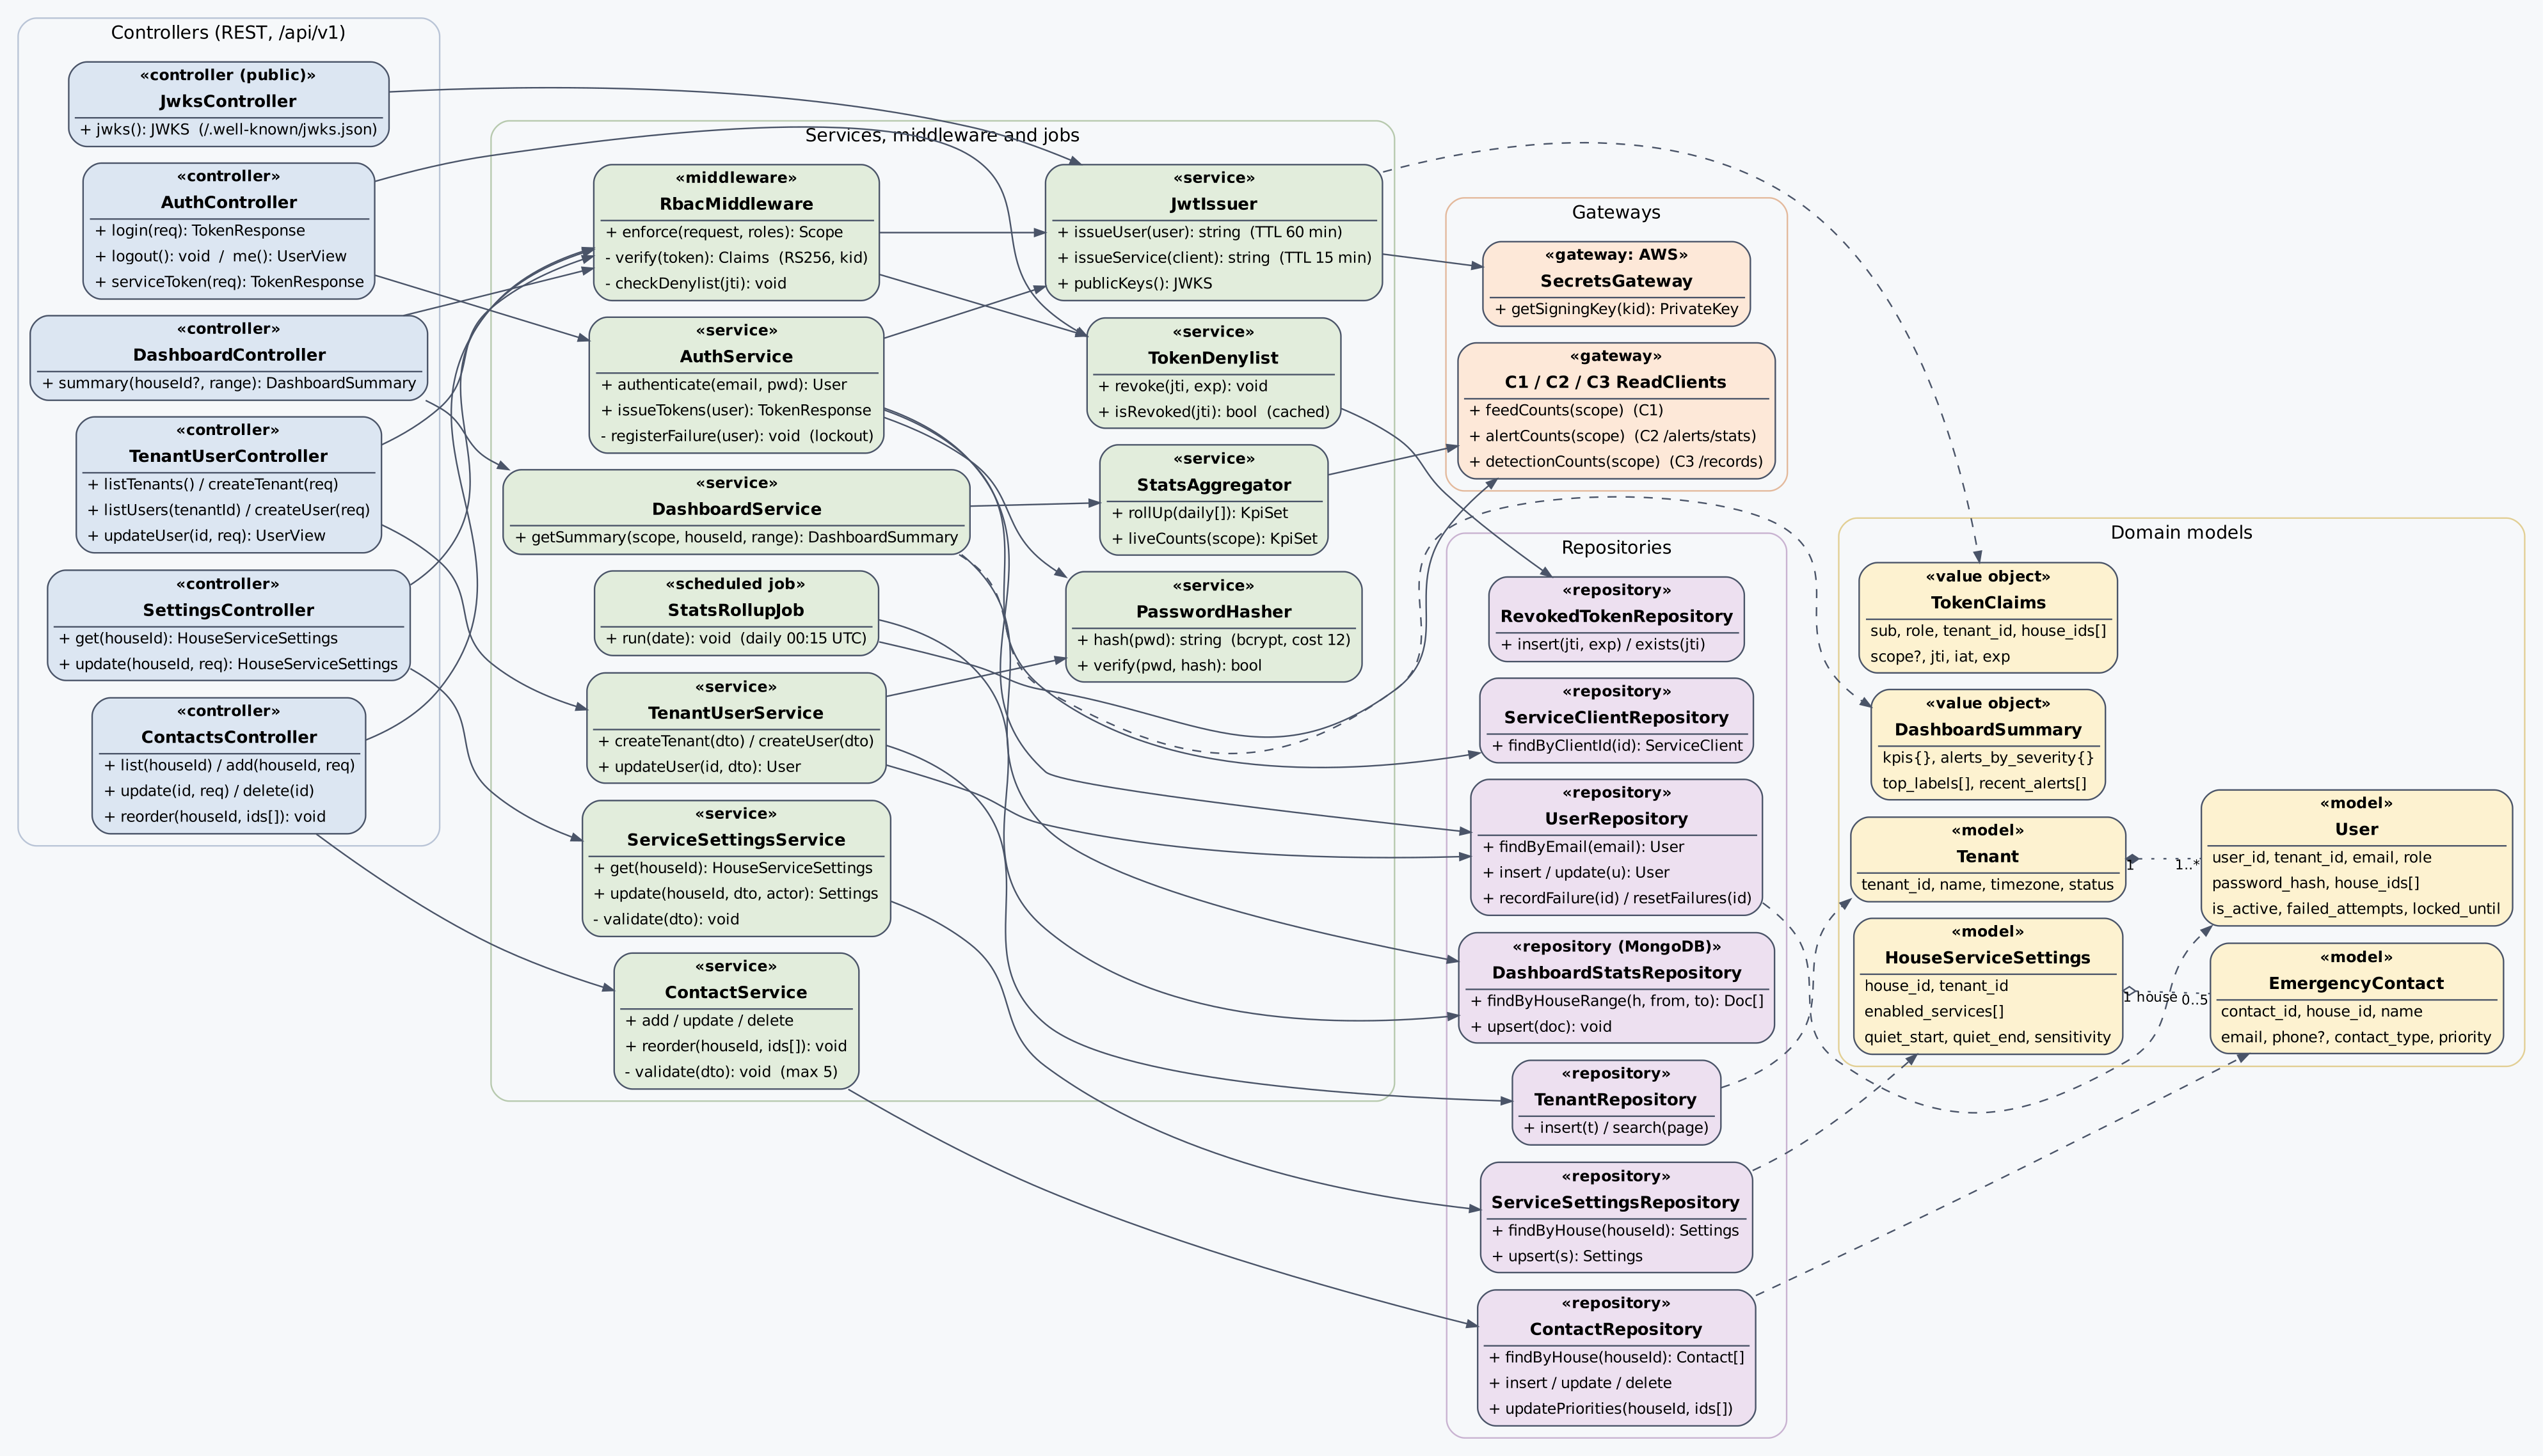
\includegraphics[width=\linewidth,height=0.86\textheight,keepaspectratio]{figures/C4/c4-class}
\captionof{figure}{C4 internal class diagram: controllers, auth and RBAC, dashboard and settings services, repositories, gateways and models}\label{fig:c4-class}
\end{landscape}

\begin{longtable}{L{3.6cm}L{2.0cm}L{5.7cm}L{3.5cm}}
\caption{C4 class specification}\label{tab:c4-classspec}\\
\toprule
\textbf{Class} & \textbf{Type} & \textbf{Responsibility} & \textbf{Uses} \\
\midrule
\endfirsthead
\caption[]{C4 class specification (continued)}\\
\toprule
\textbf{Class} & \textbf{Type} & \textbf{Responsibility} & \textbf{Uses} \\
\midrule
\endhead
\texttt{RbacMiddleware} & middleware & Verify, check denylist, check role and house, attach scope & \texttt{JwtIssuer}, \texttt{TokenDenylist} \\
\texttt{AuthService} & service & Login, lockout, service-client auth & \texttt{UserRepository}, \texttt{PasswordHasher}, \texttt{JwtIssuer} \\
\texttt{JwtIssuer} & service & Sign RS256 tokens; publish JWKS & \texttt{SecretsGateway} \\
\texttt{TokenDenylist} & service & Revoked \texttt{jti} until expiry (cached) & \texttt{RevokedToken\allowbreak Repository} \\
\texttt{DashboardService} & service & Scoped summary for house and range & \texttt{StatsAggregator}, \texttt{DashboardStats\allowbreak Repository} \\
\texttt{StatsAggregator} & service & Merge daily docs and live counts & C1/C2/C3 read clients \\
\texttt{StatsRollupJob} & job & Nightly per-house daily document & read clients, stats repository \\
\texttt{ServiceSettings\allowbreak Service}, \texttt{ContactService} & service & Validate and save settings and contacts & settings and contact repositories \\
\texttt{TenantUserService} & service & Tenants and users; password hashing & tenant and user repositories \\
\bottomrule
\end{longtable}

\subsection{Data and database design}
C4 owns six PostgreSQL tables and the \texttt{dashboard\_stats\_daily} MongoDB collection (Figure~\ref{fig:c4-er}).

\figH{C4/c4-er}{0.9}{C4 entity-relationship diagram}{fig:c4-er}

\begin{longtable}{L{4.4cm}L{3.0cm}L{7.2cm}}
\caption{C4 data dictionary (key fields)}\label{tab:c4-dd}\\
\toprule
\textbf{Table.column} & \textbf{Type} & \textbf{Constraint / description} \\
\midrule
\endfirsthead
\caption[]{C4 data dictionary (key fields) (continued)}\\
\toprule
\textbf{Table.column} & \textbf{Type} & \textbf{Constraint / description} \\
\midrule
\endhead
\texttt{users.role} & VARCHAR CHECK & \texttt{house\_owner}, \texttt{iot\_staff}, \texttt{cloud\_staff} \\
\texttt{users.password\_hash} & VARCHAR(100) & bcrypt hash; never returned by any API \\
\texttt{users.house\_ids} & UUID[] & Houses (C1) an owner may see; empty for staff \\
\texttt{users.failed\_attempts}, \texttt{locked\_until} & SMALLINT, TIMESTAMPTZ & Lockout state \\
\texttt{house\_service\_settings.enabled\_services} & TEXT[] & Service codes; C2 \texttt{alert\_types.service\_code} references these \\
\texttt{house\_service\_settings.quiet\_start/end} & TIME NULL & House local time; may wrap midnight \\
\texttt{house\_service\_settings.sensitivity} & VARCHAR CHECK & \texttt{low}, \texttt{medium}, \texttt{high} (Table~\ref{tab:c4-dt-sens}) \\
\texttt{emergency\_contacts.priority} & SMALLINT & 1..5, UNIQUE (house\_id, priority) DEFERRABLE \\
\texttt{emergency\_contacts.contact\_type} & VARCHAR CHECK & \texttt{family}, \texttt{caregiver}, \texttt{neighbor}, \texttt{emergency\_service} \\
\texttt{service\_clients.scopes} & TEXT[] & Allowed scopes per component \\
\texttt{revoked\_tokens.jti} & UUID PK & Purged after \texttt{expires\_at} \\
\texttt{dashboard\_stats\_daily.\_id} & string & \texttt{house:date}; counts by severity, label, clips, feeds \\
\bottomrule
\end{longtable}

\subsection{Program function descriptions}
\begin{longtable}{L{4.0cm}L{4.0cm}L{6.6cm}}
\caption{C4 key internal functions}\label{tab:c4-fn}\\
\toprule
\textbf{Function} & \textbf{Inputs $\rightarrow$ outputs} & \textbf{Logic} \\
\midrule
\endfirsthead
\caption[]{C4 key internal functions (continued)}\\
\toprule
\textbf{Function} & \textbf{Inputs $\rightarrow$ outputs} & \textbf{Logic} \\
\midrule
\endhead
\texttt{AuthService.\allowbreak authenticate} & email, password $\rightarrow$ User & Lockout check, bcrypt verify, failure counting \\
\texttt{JwtIssuer.\allowbreak issueUser} & User $\rightarrow$ token & Claims + \texttt{jti}, 60 min, RS256 with current \texttt{kid} \\
\texttt{RbacMiddleware.\allowbreak enforce} & request, roles $\rightarrow$ scope & Verify, denylist, role, house \\
\texttt{ContactService.\allowbreak reorder} & house, ids $\rightarrow$ void & All ids present once; priorities 1..n in one transaction \\
\texttt{DashboardService.\allowbreak getSummary} & scope, house, range $\rightarrow$ KPIs & Daily docs for past days + live counts for today \\
\texttt{StatsRollupJob.\allowbreak run} & date $\rightarrow$ void & Per house: counts from C1/C2/C3; upsert \\
\bottomrule
\end{longtable}

\figH{C4/c4-login-rbac-flow}{0.64}{Login and RBAC flowchart: verify credentials, issue the scoped token, then verify and scope every later request}{fig:c4-flow}

\begin{Shaded}
\begin{Code}
function authenticate(email, password):
    user = users.findByEmail(lower(email))
    if user and user.locked_until and now() < user.locked_until: raise 423 account_locked
    if user is None or not user.is_active or not bcrypt.verify(password, user.password_hash):
        if user: users.recordFailure(user.id)          # 5 failures in 15 min -> locked_until = now + 15 min
        raise 401 invalid_credentials
    users.resetFailures(user.id)
    return user

function issueUser(user):
    claims = { sub: user.id, role: user.role, tenant_id: user.tenant_id, house_ids: user.house_ids,
               jti: uuid4(), iat: now(), exp: now() + 60 min }
    return rs256Sign(claims, secrets.getSigningKey(CURRENT_KID), kid=CURRENT_KID)

function enforce(request, allowedRoles, houseId=None):
    claims = rs256Verify(request.bearer, jwks)          ; if invalid or expired: raise 401 token_expired
    if denylist.isRevoked(claims.jti):                  raise 401 token_revoked
    if claims.role not in allowedRoles:                 raise 403 forbidden
    if houseId and claims.role == "house_owner" and houseId not in claims.house_ids: raise 403 forbidden
    request.scope = Scope(claims.tenant_id, claims.house_ids, claims.role)      # every query filters on it
\end{Code}
\end{Shaded}

\subsection{Behavior: session state machine}
Figure~\ref{fig:c4-state}: a visitor is unauthenticated until login succeeds; an authenticated request outside the
role or scope returns 403; expiry or logout returns the user to the login page on the next call.

\figH{C4/c4-session-state}{0.9}{Session and token lifecycle: unauthenticated, authenticated, access denied, expired}{fig:c4-state}

\subsection{Behavior: sequence diagrams}
Figure~\ref{fig:c4-seq} is login with role redirect followed by a scoped dashboard read (UC-08). Figure~\ref{fig:c4-seq-settings}
is an owner saving settings and reordering contacts, and C2 reading them at the next evaluation.

\figH{C4/c4-seq-login-dashboard}{1.0}{Sequence (a): login with role redirect, then a scoped dashboard summary}{fig:c4-seq}
\figH{C4/c4-seq-settings}{0.95}{Sequence (b): owner updates service settings and contact order; C2 reads them later}{fig:c4-seq-settings}

% ============================================================================
\section{Component Business Logic}

\subsection{RBAC access decision table}
\begin{longtable}{L{3.0cm}L{3.4cm}L{4.2cm}L{4.0cm}}
\caption{RBAC by role}\label{tab:c4-dt-rbac}\\
\toprule
\textbf{Role} & \textbf{Houses visible} & \textbf{May change} & \textbf{Landing page} \\
\midrule
\endfirsthead
\caption[]{RBAC by role (continued)}\\
\toprule
\textbf{Role} & \textbf{Houses visible} & \textbf{May change} & \textbf{Landing page} \\
\midrule
\endhead
\texttt{house\_owner} & own \texttt{house\_ids} & own settings and contacts; act on own alerts & Home Overview (\texttt{/home/*}) \\
\texttt{iot\_staff} & all of own tenant & houses, rooms, feeds (C1) & Camera Feed Manager (\texttt{/iot/*}) \\
\texttt{cloud\_staff} & all tenants & rules (C2), tenants, users, any settings & System Dashboard (\texttt{/ops/*}) \\
external recipient & one alert via signed link & nothing & read-only Alert View (C2) \\
\bottomrule
\end{longtable}

\subsection{Login decision table}
\begin{longtable}{L{2.2cm}L{2.0cm}L{2.2cm}L{2.6cm}L{5.4cm}}
\caption{Login outcome}\\
\toprule
\textbf{User found} & \textbf{Active} & \textbf{Locked} & \textbf{Password OK} & \textbf{Result} \\
\midrule
\endfirsthead
\caption[]{Login outcome (continued)}\\
\toprule
\textbf{User found} & \textbf{Active} & \textbf{Locked} & \textbf{Password OK} & \textbf{Result} \\
\midrule
\endhead
no & -- & -- & -- & 401 \texttt{invalid\_credentials} \\
yes & no & -- & -- & 401 \texttt{invalid\_credentials} \\
yes & yes & yes & -- & 423 \texttt{account\_locked} \\
yes & yes & no & no & 401; failures + 1; 5th in 15 min locks 15 min \\
yes & yes & no & yes & 200 token; failures reset; landing by role \\
\bottomrule
\end{longtable}

\subsection{House sensitivity to confidence adjustment}
C4 stores the sensitivity; C2 applies it to every rule's minimum confidence when it evaluates a detection.
\begin{longtable}{L{3.0cm}L{5.4cm}L{6.0cm}}
\caption{Sensitivity adjustment (applied by C2, clamped to 0.05--0.95)}\label{tab:c4-dt-sens}\\
\toprule
\textbf{House sensitivity} & \textbf{Rule min\_confidence} & \textbf{Result} \\
\midrule
\endfirsthead
\caption[]{Sensitivity adjustment (applied by C2, clamped to 0.05--0.95) (continued)}\\
\toprule
\textbf{House sensitivity} & \textbf{Rule min\_confidence} & \textbf{Result} \\
\midrule
\endhead
\texttt{low} & $+0.10$ & Fewer, higher-confidence alerts \\
\texttt{medium} & unchanged & Default \\
\texttt{high} & $-0.10$ & More, earlier alerts \\
\bottomrule
\end{longtable}

\subsection{Service and quiet-hours eligibility}
C4 stores these settings; C2 enforces them. Critical and high alerts bypass quiet hours.
\begin{longtable}{L{2.6cm}L{2.8cm}L{3.0cm}L{6.0cm}}
\caption{Alert eligibility}\label{tab:c4-dt-quiet}\\
\toprule
\textbf{Service on} & \textbf{In quiet hours} & \textbf{Severity} & \textbf{Eligible to alert} \\
\midrule
\endfirsthead
\caption[]{Alert eligibility (continued)}\\
\toprule
\textbf{Service on} & \textbf{In quiet hours} & \textbf{Severity} & \textbf{Eligible to alert} \\
\midrule
\endhead
no & -- & -- & No (\texttt{service\_disabled}) \\
yes & yes & medium, low & No (\texttt{quiet\_hours}) \\
yes & yes & critical, high & Yes (bypass) \\
yes & no & any & Yes \\
\bottomrule
\end{longtable}

\subsection{Contact validation decision table}
\begin{longtable}{L{2.4cm}L{2.4cm}L{2.6cm}L{2.6cm}L{4.4cm}}
\caption{Add contact}\label{tab:c4-dt-contacts}\\
\toprule
\textbf{Email valid} & \textbf{Unique in house} & \textbf{Count $<$ 5} & \textbf{Caller in scope} & \textbf{Result} \\
\midrule
\endfirsthead
\caption[]{Add contact (continued)}\\
\toprule
\textbf{Email valid} & \textbf{Unique in house} & \textbf{Count $<$ 5} & \textbf{Caller in scope} & \textbf{Result} \\
\midrule
\endhead
-- & -- & -- & no & 403 \\
no & -- & -- & yes & 422 \texttt{email} \\
yes & no & -- & yes & 409 \texttt{email\_exists} \\
yes & yes & no & yes & 409 \texttt{contact\_limit} \\
yes & yes & yes & yes & 201; priority = last + 1 \\
\bottomrule
\end{longtable}

% ============================================================================
\section{Component Graphic User Interface Design}

\subsection{GUI style}
\begin{longtable}{L{3.0cm}L{11.8cm}}
\caption{C4 GUI style}\\
\toprule
\textbf{Element} & \textbf{Rule} \\
\midrule
\endfirsthead
\caption[]{C4 GUI style (continued)}\\
\toprule
\textbf{Element} & \textbf{Rule} \\
\midrule
\endhead
Shell & React SPA with Tailwind; C4 provides the app shell, sidebar, breadcrumb and route guard that every component's pages render inside. \\
Route guard & Reads the JWT role; a user who opens another role's URL is sent to their own landing page; a 401 returns to login. \\
Charts & Recharts; every chart has a table fallback and labelled values. \\
Encoding & Severity and status always as icon + word, never colour alone. \\
Forms & Inline validation from 422 \texttt{details}; unsaved-changes bar with Save and Discard. \\
Accessibility & WCAG 2.1 AA, keyboard reorder for contacts (move up / down buttons as well as drag). \\
\bottomrule
\end{longtable}

\subsection{Storyboard}
Figure~\ref{fig:c4-story}: path~A is sign-in, token issue, role landing and the System Dashboard (1--4). Path~B is an
owner opening Services and Settings, toggling services and quiet hours, ordering contacts and saving (5--8).

\figH{C4/c4-storyboard}{1.0}{C4 storyboard: sign-in by role and owner configuration}{fig:c4-story}

\subsection{Function partition tree}
\figH{C4/c4-gui-tree}{0.8}{C4 GUI function partition across the three role workspaces}{fig:c4-gui-tree}

\subsection{UI markup diagram and wireframes}
Figure~\ref{fig:c4-wf-settings} is the owner's Services and Settings page with markup callouts
(Table~\ref{tab:c4-markup}); Figure~\ref{fig:c4-wireframe} is the System Dashboard for cloud staff (SRS Figure 4).

\figH{C4/c4-wireframe-settings}{0.88}{UI markup of Services and Settings (house\_owner)}{fig:c4-wf-settings}

\begin{longtable}{L{0.6cm}L{3.2cm}L{2.6cm}L{4.0cm}L{4.2cm}}
\caption{Services and Settings markup legend}\label{tab:c4-markup}\\
\toprule
\textbf{\#} & \textbf{Element} & \textbf{Template} & \textbf{Data source} & \textbf{Behaviour} \\
\midrule
\endfirsthead
\caption[]{Services and Settings markup legend (continued)}\\
\toprule
\textbf{\#} & \textbf{Element} & \textbf{Template} & \textbf{Data source} & \textbf{Behaviour} \\
\midrule
\endhead
1 & Navigation, house picker & AppShell & JWT \texttt{house\_ids} & Only own houses listed \\
2 & Detection services & ToggleTable & \texttt{GET .../settings} & One switch per service code \\
3 & Quiet hours, sensitivity & TimeRange, Segmented & settings & Note: critical and high always delivered \\
4 & Emergency contacts & SortableList & \texttt{GET .../emergency-contacts} & Drag or keyboard reorder; max 5 \\
5 & Save bar & SaveBar & \texttt{PUT .../settings}, \texttt{PUT .../order} & Shows unsaved count; 422 inline \\
\bottomrule
\end{longtable}

\figH{C4/c4-wireframe-dashboard}{0.8}{System Dashboard (cloud\_staff): KPI tiles, severity and label charts, recent alerts}{fig:c4-wireframe}

\subsection{GUI templates}
\begin{longtable}{L{3.0cm}L{4.2cm}L{7.6cm}}
\caption{GUI templates defined or used by C4}\\
\toprule
\textbf{Template} & \textbf{Used on} & \textbf{Props / behaviour} \\
\midrule
\endfirsthead
\caption[]{GUI templates defined or used by C4 (continued)}\\
\toprule
\textbf{Template} & \textbf{Used on} & \textbf{Props / behaviour} \\
\midrule
\endhead
AppShell + RouteGuard & every page of every component & Role-aware navigation, landing redirect, toasts \\
KpiTile & dashboards & value, label, delta, link \\
ChartCard & dashboards & Recharts bar chart with table fallback \\
DataTable, FilterBar & dashboards, users, tenants & Paging, house and range filters \\
ToggleTable, SortableList, SaveBar & Services and Settings & Switches, ordered list, unsaved-changes bar \\
\bottomrule
\end{longtable}
